\begin{landscape}
	
	
	\subsection{SE-22 Registrar estudiante (Sistema de reconocimiento facial)}
	
	\begin{figure}[htbp!]
		\begin{center}
			\fbox{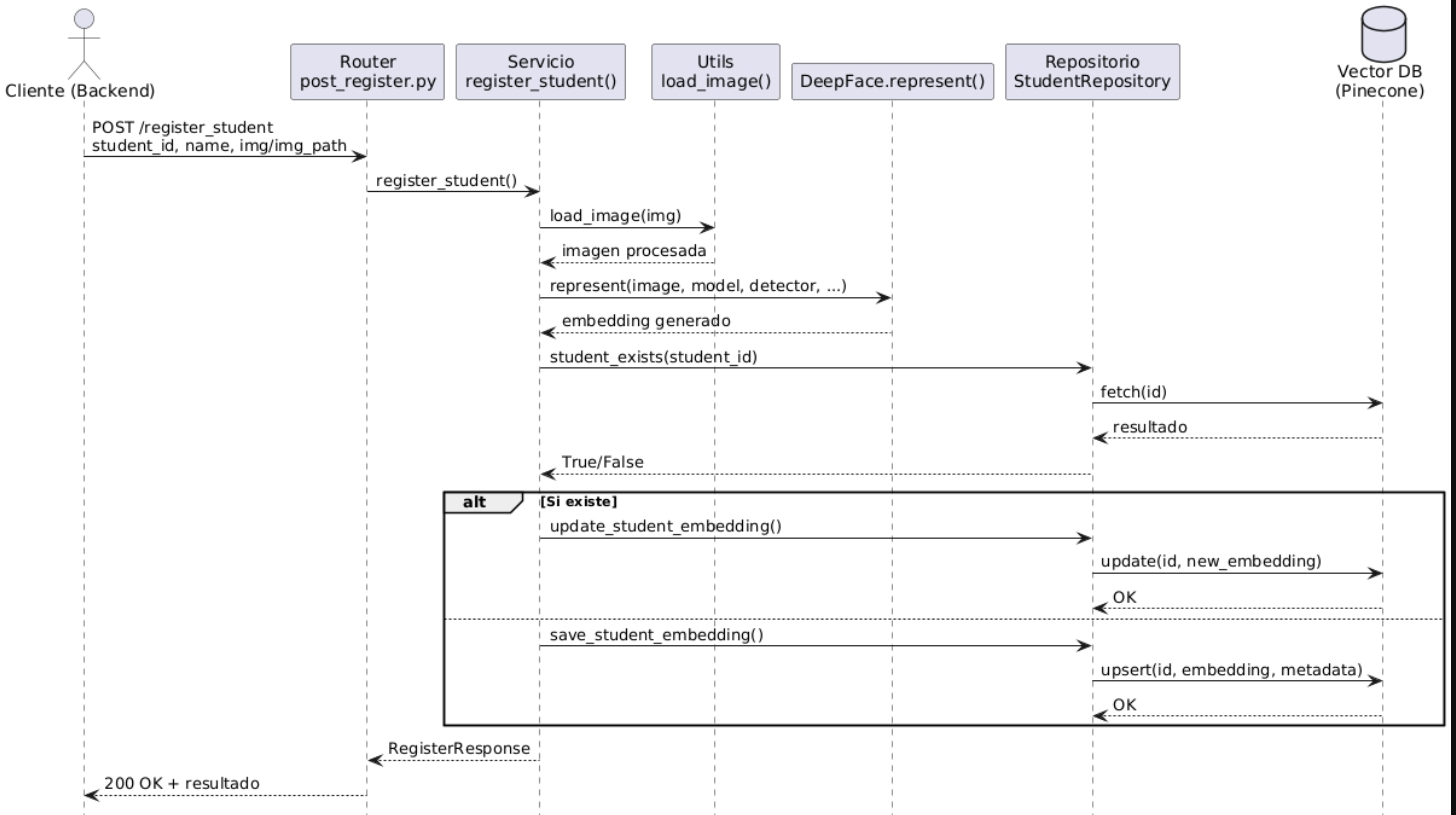
\includegraphics[width=1\textwidth]{Secuencia/RF-Register}}
			\caption{Diagrama de secuencia del endpoint register student).}
			\label{fig:Diagrama de secuencia RF-Registro}
		\end{center}
	\end{figure}
	
	En este diagrama de secuencia (figura  \ref{fig:Diagrama de secuencia RF-Registro}) se describe el proceso que sigue la lógica implementada para el sistema de reconocimiento facial cuando se necesita registrar a un estudiante, por si sola, la secuencia de pasos era muy grande para incluirla en los diagramas de secuencia que llaman a este endpoint, por lo que aquí se detalla mejor su funcionamiento.
	
\end{landscape}
